\section{Introduction}

While the degree to which the historical development of languages is inferred and used by language learners has long been of interest to sociolinguists~\citep{Labov1989}, empirically this question has only been tackled relatively recently as part of a general effort to study the acquisition of sociolinguistic knowledge by individuals~\citep{Labov2014}.
Of particular relevance to this thesis is the question of how specific linguistic variants and their relative usage levels can come to be associated with specific age groups.
The concept of `age vectors' captures the age-based stratification of variable usage, and the idea that individual language users possess knowledge of the age vectors of their community has been invoked as an explanation of how language changes are transmitted and increment across generations~\citep{Labov2001}.
The model presented in the previous chapter demonstrated how a similar mechanism, based on tracking changes to frequency distributions of discrete variants in \emph{real time}, can equally account for spontaneous directed transitions of change in a speech community.

While there is an increasing body of empirical evidence on individuals' knowledge of ongoing changes which I reviewed in Section~\ref{sec:agevector}, the experimental data presented there was limited to continuous phonetic changes. Although the fact that this sub-domain of language change still encompasses the largest part of sociolinguistic research might in part be attributed to the generativist sovereignty over morphosyntactic research which did not leave much space for an empiricist-variationist methodology, it is worth noting that the type of sociolinguistic variable (i.e.~whether different variants differ continuously or categorically) influences not just how the linguist might describe or represent variation, but also how that variation is acquired by individuals. %makes a difference, in particular when it comes to enquiring about the \emph{knowledge} about changes.

In particular, the type of variable impacts on the amount of information on inter-individual differences that can be extracted from individual realisations of a variable that is observed in an interaction. While continuous phonetic tokens are potentially very noisy and it might therefore help to have access to a speaker's full distribution of realisations to get a complete picture of their variable usage, given sufficient stratification of variable realisations along a continuous dimension even a single token can potentially contain enough information to place the speaker along a cline from `more outdated' to `more modern' in their variant usage.
Not only that, continuous variants allow speakers to sound `\emph{even more} novel' by extending the change along that cline and producing variants that `overshoot' even the most advanced novel variants, productions which can nevertheless be immediately understood as instantiations of the same innovation.
%\citep{Swarup2012}.
%figure out the age vector between them, in theory you only need as little as one token each from a younger and an older speaker which, given the relative frequency of phonetic variables, should be easy enough to get access to.

The same is not true in the case of categorical variants. Firstly, in order to learn about an individual speaker's variable usage,
%level of participation in a change
one truly need to learn about the overall distribution of realisations, i.e.~the relative frequencies with which the different variants are mixed by the speaker.
Except when different variants are strong social markers which are exclusively used by non-overlapping speaker groups, very little information can be extracted from individual productions. %realisations of a variable.
%which could theoretically be the case for really rapid changes where youngers speakers categorically use only variant that is still unattested in 
Instead, several realisations of a variable by one and the same speaker are necessary to make strong inferences about a speaker.
In combination with the fact that morphosyntactic variables can only be observed much less frequently than most phonetic and phonological ones, 
it is not obvious that people would be as good at acquiring or making inferences about categorical variables as they are for continuous ones, like the vowel realisations tested by~\citet{Drager2011}.

%one sample each you're quite likely to end up with both producing the same token, which is uninformative.

%And to come back to frequency, you also need to wait until you've collected 5+ samples of imperatives with an explicit subject before you can make strong inferences about your speaker, so

%One could argue that all our speakers are doing is learn a simple 'new variant = younger speaker, old variant = older speaker' mapping, but the difference in responses between the imperative and question variables shows that this is not the case: while the reported apparent time differences could be explained by such a simple associative mapping, the fact that the new imperative variant is reported to be used relatively less by *all* speaker groups shows that individuals actually know something about the relative usage of the variants within the individual!

%Beyond the domain of continuous phonetic change,
In one of the rare studies investigating age effects for categorical rather than continuous~(phonetic) traits, \citet{Walker2011} showed the influence of congruence between `word age' and `voice age' in facilitating lexical access: listeners of all ages exhibited a speed-up in processing words produced by a voice indicative of an age group, exactly when the word was more likely to be used by speakers of that age group. %, whether the item or referent were outdated.
Although this experiment speaks to the influence of perceived age directly, it does not involve a sociolinguistic variable, since the different stimuli belong to different semantic domains, rather than being different ways of `saying the same thing'.

%in particular with respect to how variants and usage levels 

%Most traditional accounts of language change are based on the assumption that linguistic divergence occurs during language acquisition, mostly based on language-internal factors that make learners `mislearn' or `reanalyse' their linguistic input, causing them end up with a different target language than that spoken by their caretakers~\citep[see e.g.][]{Salmons2013}. But quantitative research on infants and adolescents has painted a much more refined picture of the \emph{target} of child language acquisition~\citep{Labov2012}. Of particular relevance is the question of how individuals acquire sociolinguistic variation, and how this acquisition develops over time. Quantitative studies of the linguistic patterns of different pre-adolescent age cohorts has shown that, while children's usage patterns might mirror the idiosyncratic language use of their caretakers up until about age three or four, learners then exhibit a pronounced ``outward-orientation'': shedding most of the influence of their caretaker speech, learners instead turn not just towards their peers, but towards the usage patterns in the wider speech community as a whole~\citep{Labov2014}. % also Labov2001, ch.13

The goal of the present work is to extend the body of research on `age vectors', as they are perceived and used by the individual, to the domain of syntactic change. Since this an understudied area of research, we will also present a novel questionnaire methodology designed to help quantify people's explicit knowledge about ongoing language changes, in particular their impressions of the changes' direction.

Here, a disclaimer is in order regarding the term \emph{awareness} which, in contemporary linguistic research, is typically used to refer to an individual's explicit, \emph{meta-linguistic} knowledge about their own and their community's language use~\citep{Preston2005}. This knowledge is consequently described as being ``above the level of conscious awareness''~\citep[p.283]{Baranowski2013} of the individual. While the terminology used in this chapter reflects the fact that the present methodology is based on participants' \emph{explicit} statements about their meta-linguistic knowledge, it should be noted that conscious awareness is just one possible proxy that allows one to test individuals' ability to detect (and potentially amplify) linguistic trends. Although this chapter is dedicated exclusively to the study of linguistic \emph{awareness} of changes, the mechanism of momentum-based language change does not strictly rely on awareness per se, but would most likely be driven by implicit knowledge which could be tested through more sophisticated experimental methods such as the ones used by \citet{Drager2005,Drager2011}.

\section{Quantifying the awareness of syntactic changes}

In this work we investigate the human capacity for tracking changes in syntactic variables by probing speakers' awareness of three instances of the loss of verb movement in the variety of Scots spoken in Shetland. Shetland is a group of islands approximately 200km North of Great Britain with around 23,000 inhabitants across 15~inhabited islands~\citep[see also Figures~\ref{fig:shetlandcontext} and~\ref{fig:shetland}]{Shetland2014}. While Shetland forms part of the United Kingdom, it was only passed from Denmark to the Crown of Scotland in the late 1400s, and the islands' linguistic history is correspondingly diverse. Although virtually all toponyms on the island can be traced back to Viking origins, the Scots settlers who emigrated to the islands following the annexation to the Scottish Crown brought their own West-Germanic vernaculars with them. These vernaculars gradually replaced the local \emph{Norn} language, a North Germanic variety most closely related to Old Norwegian, which however continued to be spoken on the isles until at least the 18th century~\citep{Knooihuizen2009}. Today, the primary native vernacular of Shetland can be characterised as a variety of Scots, which is itself a continuum of language varieties spoken throughout the Scottish Lowlands that has developed largely in parallel to (rather than being derived from) the more well known English varieties that spread from England to many other parts of the globe~\citep[p.15]{Millar2007}.

\begin{figure}
\centering

\includegraphics{figure/shetlandcontext}
\caption[Shetland's location in the North Sea]{Shetland's location in the North Sea, showing the territorial waters of the United Kingdom, Norway and the Faroe Islands as well as ferry links and natural conservation areas. % Distance to Bergen + Aberdeen is 350km
Projection:~Web~Mercator. \textcopyright~\href{http://www.openstreetmap.org/copyright}{OpenStreetMap contributors}, licensed under the \href{http://creativecommons.org/licenses/by-sa/2.0/}{Creative Commons Attribution-ShareAlike 2.0 license (CC BY-SA)}.}
% 200dpi=1:5000000 (ferries and marine areas rendered)
% 150dpi=1:7500000
% convert -density 150 -units pixelsperinch in.png out.png
\label{fig:shetlandcontext}
\end{figure}

\begin{figure}
% width=412.56497pt height=629.82918pt
% 6 lines: 0.1925378, 7 lines: 0.1865378
%./remap.py -x ling-Shetland.xml --scale 600910 --width 0.1449794 --height 0.1915378 -o /home/kevin/thesis/questionnaire/figure/shetland.pdf
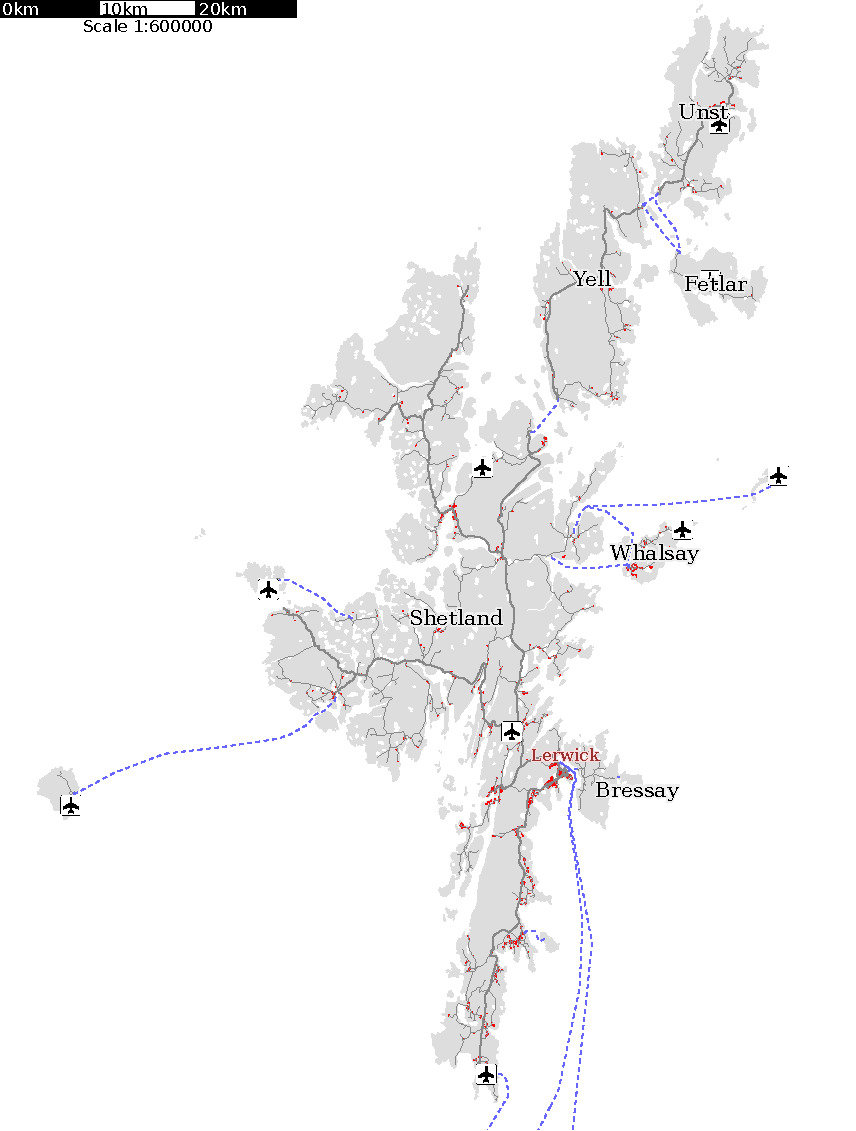
\includegraphics{figure/shetland}
\caption[Detail of the Shetland archipelago]{Detail of the Shetland archipelago showing paved roads, ferry routes, airports and areas of human residence~(in~red). Ferry connections to the Scottish mainland leave from the capital town of Lerwick, also the largest settlement. Regular flights to several Scottish airports as well as Bergen~(Norway) depart from Sumburgh Airport at the Southern tip of the main island, with many more airfields for local planes scattered across the archipelago. Projection:~orthographic, centered on 60.345\textdegree N and 1.4\textdegree W. Map data~\textcopyright~OpenStreetMap contributors.}
\label{fig:shetland}
\end{figure}

Due to its insular location and sustained contact with North Germanic languages~\citep{Jamieson2016}, Shetland Scots has retained many linguistic features typical of Germanic languages that the varieties of English and Scots on the British mainland have long lost. Some examples which will be evident in the questionnaire examples below are the relatively rich verbal inflection, as well as the maintenance of a number distinction in the second person pronoun \emph{du}~(cognate with Middle English \emph{thou}). The features under investigation in this study are also of the historically conservative kind, namely the inversion of the verb position in several syntactic contexts, all of which occur alongside the emergence of periphrastic \emph{do} (or `do-support').
While for most areas of England the change away from the historically original verb-initial constructions~\citep[see][for a more detailed analysis]{Jamieson2015} can be dated to the period from 1500-1700~\citep{Ellegard1953,Kroch1989do}, the homologous change in Shetland Scots has only been unfolding over the course of the 20th century~\citep{Jonas2002}. % Millar2007 p.76
The three related changes currently ongoing in Shetland which we investigate in the current work are as follows:

\begin{itemize}
\item verb positioning in imperatives, which is changing from a raised verb (surface realisation \texttt{VSO}) to Standard English \texttt{SVO} structure. An example in Shetland Scots would be ``Mak du dy ain denner!'' vs. ``Du mak dy ain denner!'', with the latter (incoming) variant akin to Standard English syntax, i.e.~`You~(sg.) make your~(sg.) own dinner!'

\item yes/no question syntax: change from a main verb-initial to a `periphrastic do' structure, e.g. from ``Kens du Sarah?'' to ``Does du ken Sarah?'', with `ken' being the Scots lexeme for `to know'.

\item wh question syntax: change from plain \texttt{WhVSO} with a fronted main verb to a `periphrastic do' structure, i.e. \texttt{Wh-`do'-SVO}. An example of the two constructions would be old ``Whit gae du him?'' to ``Whit did du gie him?'', with `gie'/`gae' the Scots equivalents of Standard English `give'/`gave'.
\end{itemize}

In all three cases, usage of the incoming variants is already common. The two question variables are more advanced, with younger speakers almost categorically using the incoming variants~(with the exception of a few lexically specific items, see \citealt{Jamieson2015}).
% see also a current assessment of acceptability in 
So while the changes are in a sense nearing completion, all members of the speech community are still exposed to both outgoing and incoming variants due to their being used frequently by older speakers.

\subsection{Methodology}\label{sec:questionnaire}

To quantify people's explicit knowledge about ongoing language changes we adapted a self-evaluation method originally used to investigate the perception of phonetic changes by \citet{Labov1966} and \citet{Trudgill1972}, who asked speakers to report their relative usage of several phonetic variables. We refined the methodology, so that every sociolinguistic variable under investigation was covered by a one page questionnaire eliciting speakers' estimates of their own usage, as well as that of other social groups, alongside other (folk-)linguistic beliefs about the linguistic variants themselves\footnote{The complete materials of the paper-based questionnaire can be found in Appendix~\ref{app:questionnaire}.}. At the top of each questionnaire page, the two competing syntactic variants were introduced in the following way:

\begin{framed}
\begin{center}
You are probably familiar with these two ways of asking somebody to do something:\\
``\emph{Mak du dy ain denner!''\hspace{3cm}``Du mak dy ain denner!''}
\end{center}
\end{framed}

The order of the two variants was randomised between individuals, in the above example the outgoing variant is on the left, the incoming one (akin to Standard English ``You make your own dinner!'') on the right. The dialectal spelling of the example sentences is quasi-standardised on Shetland, and their mixing with the Standard English formulations of the questionnaire is not unusual. The actual questionnaire consisted of the following five questions~(referred to as \emph{Q1} through \emph{Q5} throughout the text) which were intended to probe different aspects of people's explicit knowledge about the changes in question:

% How much do you use either of these variants? \begin{likert}\begin{tabular}{ x x x x x } $\square$ & $\square$ & $\square$ & $\square$ & $\square$ \\ I use only `Mak~du..' & I use more `Mak~du..' & I use both equally & I use more `Du~mak..' & I use only `Du~mak..' \end{tabular}\end{likert}

\begin{description}
\item[Question 1:] ``How much do you use either of these variants?'' \hfill \\ This explicit question regarding speakers' own frequency of use could be answered on a 5-point scale, with the options labelled `I use only~(variant 1)', `I use mostly~(variant 1)', `I use both equally', `I use mostly~(variant 2)' and `I use only~(variant 2)', with the order of the two variants matching those of their initial presentation at the top of the page. % This information can be correlated with grammaticality judgments
\item[Question 2:] ``How much do you think are people around you using either of the variants?'' \hfill \\ This question could again be answered on a 5-point scale with options `People use only~(variant 1/2)/mostly~(variant 1/2)/both equally'. This question does not just provide information on speakers' perception of their average interlocutors' frequency of use, but the \emph{relative difference} between the answers to questions 1 and 2 can potentially provide information on whether speakers think of themselves as being `ahead' or `behind' the curve of a particular change relative to their speech community. % (but see results)
\item[Question 3:] ``Which of the two variants do you think is \emph{older}?'' \hfill \\ This (intentionally vague) question is intended to get at speakers' beliefs or connotations regarding the `age' of the competing variants, without drawing explicit attention to the fact that the variable is in fact changing. The three possible answers were `(variant~1) is older', `(variant~2) is older' and `People have always used both', with the order of the two variants randomised.
\item[Questions 4+5:] ``How much do you think \emph{younger/older speakers} use either of the variants?'' \hfill \\ The final two questions tap into speakers' awareness of the apparent time development of a change, with the same 5-point options as above: `Younger/older speakers use only~(variant 1/2)/mostly~(variant 1/2)/both equally'. The order of the two questions was randomised between individuals.
\end{description}

Data collection proceeded in three stages: first, to pilot the methodology, 8~participants were asked to complete the paper version of the questionnaire on site in Shetland in January 2015. The pilot questionnaire consisted of just two sociolinguistic variables with the following example sentences:

\begin{enumerate}
\item verb positioning in imperatives: \emph{Mak du dy ain denner!} vs. \emph{Du mak dy ain denner!}, with the latter (incoming) variant akin to Standard English syntax, i.e.~`You~(sg.) make your~(sg.) own dinner!'
\item negation marking: \emph{He didna go} vs. \emph{He didnoo go} -- this sociolinguistic variable is not undergoing change and was added as a control, with `didna' being the negation variant used categorically in most of Shetland, set against the `didnoo' variant which is categorical only on the island of Whalsay to the East of Shetland's main island~(see Figure~\ref{fig:shetland}). With a population of around 1,000 and close links to the mainland, we expected the local `didnoo' variant (as well as its geographical patterning) to be known to all Shetland locals, an assumption that was borne out by several explicit references to the the variants' distribution by locals during data collection. %, this variable is related to the negation via \emph{na} vs. \emph{no} in mainland Scots).
\end{enumerate}

Following the successful pilot, 16 more participants were asked to complete an extended 4-page version of the questionnaire which covered two further variables:

\begin{enumerate}
\setcounter{enumi}{2}
\item yes/no question syntax: \emph{Kens du Sarah?} vs. \emph{Does du ken Sarah?}, i.e. ``Do you~(sg.) know Sarah?'', with `ken' being the Scots lexeme for `to know'
\item wh question syntax: \emph{Whit gae du him?} vs. \emph{Whit did du gie him?}, the latter again akin to Modern English syntax but with the Scots lexical items for Standard English `what' and `give'.
\end{enumerate}

These first 24 participants were part of a balanced sample matched for binary gender, age, and geographic location within Shetland. All participants grew up in and were currently living in rural locations in Shetland~(i.e.~outside the island's main town, Lerwick). Participants had on average spent 3.7 years living away from Shetland, typically for higher education, work or training purposes. In all cases, the questionnaire was administered as an exit-questionnaire following a $\approx40$~minute task which involved providing grammaticality judgments for a large number of examples of the changing variables in question as well as fillers, which was carried out in pairs~(see~\citealt{Jamieson2015} for a full description of the methodology and analysis of results). % with the researcher being a Shetland local

Finally, we created an identical online version of the 4-variable questionnaire which was advertised via email and social networks. The online questionnaire was self-contained (i.e.~not preceded by the grammaticality judgment task) and provided us with a convenience sample of another 53 participants from all over Shetland, who completed the questionnaire in April 2015\footnote{The online version of the questionnaire is still available for reference at \url{http://spellout.net/ibexexps/kstadler/shetland/experiment.html}.}.
%Apart from their age, gender and current geographical location we also collected information on all participants' occupation, where in Shetland they grew up, any extended times they spent outside the isles, as well as the origin of their parents.

\subsection{Hypotheses \& predictions}\label{sec:questionnairepredictions}

Based on previous research on both the specific syntactic changes under investigation as well as sociolinguistic knowledge more generally, we can derive several predictions about what effects we might expect so see \emph{a priori}.

Regarding differences between the sociolinguistic variables, prior work on verb inversion in Shetland as well as the results derived from the acceptability judgments reported in \citet{Jamieson2015} suggests that the two question variables should pattern differently from the imperatives. The change in question syntax is more advanced, with younger speaker using the incoming question variants almost exclusively. Across the population, we would therefore expect generally higher incoming variant usage for those two variables, as opposed to still relatively mixed usage of the two imperative variants. This general pattern should be observable to different degrees across all of our questions related to usage rates, i.e.~all questions but Q3.

If our informants are indeed aware of the ongoing changes and their directionality, this should be evident in their responses to questions 3 through~5. Here, all three changing variables under investigation should pattern differently from the stable negation variable which acts as our control: since this variable is not undergoing change, it provides us with a baseline for responses to explicit questions about variant age when variable usage is really patterned geographically rather than temporally. % (as far as we can tell none of the studies of sociophonetic knowledge about age reported results from non-changing baseline phonemic distinctions)

In terms of between-participant differences, we can test a number of hypotheses that are implicit in much contemporary sociolinguistic research: because many studies of sound changes in progress have found there to be a significant effect of gender (typically with females leading a change), it has been argued that, primarily due to their position in Western societies, women might be more sensitive to linguistic cues~(\citealt{Trudgill1972}, but see~\citealt{Eckert1989,Labov1990}). While the studies of automatic implicit sociophonetic knowledge discussed above have not revealed any effect of gender, \citet{Carrera-Sabate2014} showed that % based on explicit elicitation
young females were more explicitly aware of an ongoing sound change in the Lleidatà dialect of Catalan. Although no gender differences have been reported for the current syntactic changes in Shetland, neither in production nor in terms of grammatical acceptability~\citep{Jamieson2015}, we can still assess the claim that female speakers might be more sensitive or aware of ongoing changes.

Another interesting question regarding between-speaker differences pertains to how the sociolinguistic knowledge of age patterning might differ between participants of different ages. For example, in her experiment \citet{Drager2011} found an effect of listener \emph{age}, where only \emph{older} participants' perception of vowels that were currently undergoing a chain shift were affected by the perceived age of the speaker whose tokens they were asked to classify. In other words, older speakers were actively compensating more strongly for the manipulated age difference, with younger speakers exhibiting less sociophonetic sensitivity, at least in the sense that they were not actively employing their knowledge of ongoing changes in the classification task. Although we should consider the possibility that the age of our participants will affect their sociolinguistic knowledge of the variables under investigation in this work, it is not possible to derive a straightforward prediction regarding the presence or direction of an effect from the literature. While age effects are also attested in the large body of empirical research on language \emph{attitudes}~\citep{Giles2004}, it is not immediately obvious how and whether the \emph{qualitative} evaluation of innovations (often assumed to be primarily negative, see e.g.~\citealt{Labov2001,Tagliamonte2012}) corresponds to the \emph{quantitative} evaluation and perception of changes, with currently no conclusive results regarding the effect of age on the latter. % We will return to the question of research methodology below.

\section{Results}

Pooling together the data from the paper-based and online questionnaires, the total number of responses was~$N=77$ for the imperative~(\texttt{imp}) and negation~(\texttt{neg}) variables, and~$N=69$ for the yes/no question~(\texttt{ynq}) as well as wh question~(\texttt{whq}) syntax. Both the locally collected and online samples had a similar age distribution, with participants ranging from 18 to 73 years, with a median age of 32.

%round(mean(subset(participants, condition=="online")$age))/round(mean(subset(participants, condition=="paper")$age)), median age median(subset(participants, condition=="online")$age)/r median(subset(participants, condition=="paper")$age)



\begin{figure}[htbp]

{\centering \includegraphics[width=\maxwidth]{figure/questionnairelocation-1} 

}

\caption[Origin of questionnaire participants within Shetland, by condition]{Origin of questionnaire participants within Shetland, by condition~(online convenience sample vs. paper-based controlled sample)}\label{fig:questionnairelocation}
\end{figure}



In terms of the geographical location of our participants there was a bigger difference between the two samples, as can be seen in Figure~\ref{fig:questionnairelocation}. The balanced sample explicitly excluded speakers originally from Shetland's capital Lerwick, home to 7,500 of the islands' total population of 23,000. The Scots vernacular of Lerwick is undergoing a more rapid change towards Standard Scottish English~(SSE) forms than rural variants~\citep{Sundkvist2011}, a development that can be attributed to the larger influx of speakers of other English varieties due to the capital's role as a hub for offshore oil drilling in the surrounding sea.
% For example, the outgoing verb-initial constructions for questions are not attested even in older speakers from Lerwick~(Durham, p.c.).
The convenience sample on the other hand naturally includes a large proportion of Lerwick respondents. However, when it comes to their questionnaire responses, we did not find the Lerwick participants to pattern differently from the rest of the population for any of the questions.
%Even though we collected some information on the socio-economic status of our participants (in particular their profession), this data is of a qualitative nature and will therefore not be used in our statistical models.
%We will go through the results question by question.

Also, despite the fact that we might have expected the on-site participants to be more aware or sensitive to the questionnaire based on the preceding 40~minute acceptability judgment task on related syntactic variables, the type of data collection (paper-based on site vs. online) did not come out as a significant predictor in any of the statistical models reported below.

% TODO correlation between per-individual responses to the three variables?

\subsection{Assessing the reliability of subjective usage judgments}\label{sec:judgmentcorrelation}

Before we turn to the actual data analysis, we have to address a central issue of our methodology, namely the type of data collected and its reliability. While questionnaires are still one of the standard tools employed in dialectological research, explicit questions about language use have fallen into disfavour in the quantitative sociolinguistic tradition. One reason for this is that lay-people's subjective evaluation of linguistic forms is traditionally not regarded as a reliable indicator of usage, as overt evaluations are often assumed to reflect the participants' qualitative sociolinguistic attitudes rather than people's actual quantitative usage~(Labov, Trudgill, inter alia).
%With the topic of language attitudes established as a research area in its own right, in combination with
In combination with the increased availability of speech and text data analysis technology over the past few decades, the relevance of subjective data on language use outside dedicated areas of research such as language attitudes has all but disappeared.
There has, however, been a recent re-increase in interest in the beliefs that non-linguists have about language variation which bridges the two fields, with its own research methodologies often referred to as \emph{perceptual dialectology}~\citep{Montgomery2011}. % to which the current work can also be attributed.
Rather than completely discarding the opinions of laypersons on the topic of language, this approach raises a number of own research questions regarding how naive speakers' `folk beliefs' about language are related to language use as studied by linguists~\citep{Preston1996}.

It is in this domain that broadly sociolinguistic approaches come closer to the methodologies still most frequently used to study syntax and syntactic variation, in particular by means of \emph{grammaticality judgments} which have over the years been replaced by more gradual \emph{acceptability judgments} provided by naive native speakers rather than linguistic researchers themselves~\citep{Cornips2005}.
% http://web.stanford.edu/group/cslipublications/cslipublications/HPSG/2013/miller.pdf
Based on this continuum of related research methods based on explicit linguistic opinions expressed by speakers, there is also an increasing amount of literature on the question of actual usage is reflected in acceptability judgments and processing preferences~\citep{Sorace2005,Featherston2005} as well as attitudinal data~\citep[see e.g.][]{Maegaard2013,Durham2014}.
In order to better understand the nature of the estimated usage levels obtained through our present methodology it is therefore insightful to cross-validate the results with other measures.
% here are some pointers I got off Jim Donaldson that one could possibly go into: Miller, Arregui et al. 2006 (The Recycling Hypothesis), Gibson and Thomas 1999 (perceiving ungrammatical sentences as grammatical), Hofmeister et al. 2014 Processing effects in linguistic judgment data, Keller 2001 Gradience in grammar, Manning 2003 Probabilistic syntax, Sorace and Keller 2005 Gradience in linguistic data)
%One concern is thus that the estimated usage rates reported, particularly those concerning the speakers' \emph{own} usage, might not be representative.
% TODO general sociolinguistic focus on phonetics/data critique?
%really the question of reliability is not the only reason for the abandonment of questionnaires, it coincided nicely with a focus on high-frequency phonetic variables and the increasing availability of recording devices
%One obvious concern regarding our methodology, which draws the participants' explicit attention to the changing variables in question, is how indicative the responses are of speakers' actual usage.
While we have no quantitative production data available for the three changing syntactic variables in question which are all very low in frequency,
we can, however, compare the relative usage rates against the grammatical acceptability judgments which were collected independently for the 24~participants during the first, on site phase of data collection~(see~\citealt{Jamieson2015}). %reported by the same participants.
If the novel methodology presented here is indeed reliable, we should expect good correlation between the two measures.

Despite the fact that both grammaticality judgments and usage rate estimates were gathered through explicit elicitation, there are two big differences between the two types of data: firstly, the usage rate estimates draw explicit attention to the type of speaker that it is envisaged to be representative of, i.e.~the speaker themselves, the `average' interlocutor in their community, or a `younger' or `older' speaker specifically. This framing focusses explicitly on the variants' use in a specific context, while the acceptability judgment draws the informants' attention primarily to the linguistic variant itself.
In this way, a quantitative acceptability judgment does not distinguish in a principled manner between utterances that the informant would use in their own production, and what they would accept (or expect) from some of their interlocutors, but never actually produce themselves.

The second difference is that the usage rates as collected here capture the \emph{relative} usage of the two competing variants of a sociolinguistic variable by directly contrasting the two equivalent forms of a single example sentence. The acceptability judgments on the other hand express the \emph{absolute} acceptability of an individual example sentence on a 7-point Likert scale, without speaking directly to the \emph{relative} usage of the two competing variants.

In order to assess the reliability of our usage estimates by correlating it with the acceptability judgment data, we first need to transform the two measures to comparable scales, keeping in mind those differences. The basic idea here is to convert the absolute judgments per variant into relative ratings per variable, by comparing the per-variant ratings of the incoming and outgoing realisations of the same example sentences. Transforming the acceptability judgments to relative scores can be done in several different ways and boils down to three decisions. While none of the choices turned out to have a strong effect on the results, it is worth discussing them to get an idea of how a methodology based around acceptability judgments can be related to the present questionnaire methodology.

The first question regards exactly \emph{which} acceptability judgments should be correlated with the usage estimates. The acceptability judgment data collected by~\citet{Jamieson2015} is more abundant: each of the 24~informants provided judgments for a total of 49~example sentences across the three changing variables, covering 17~different verb types, and some of the verbs were chosen because they are known to exhibit strong lexical effects that affect the choice of syntactic construction. The two principled ways to limit the lexical effects on the acceptability measures are, on one hand, to only correlate the judgments for those sentences where the verbs match those used in the respective example sentences from the questionnaire or, alternatively, to wash out lexical effects by taking the average acceptability score over all verbs used in the acceptability judgment task. Both approaches turn out to result in almost identical correlation coefficients, and even the inclusion of all individual lexical items leads to a highly significant (if~lower) correlation coefficient.

The second decision relates to how the two acceptability judgments for the two competing variants should be converted into one measure capturing their relative acceptability, akin to the direct juxtaposition of the ``which variant do you use more'' measure employed by the questionnaire. The two most straightforward ways to combine them into one measure is by taking the difference between the ratings for the incoming and the outgoing variant, either by subtraction (absolute difference in acceptability) or division (relative difference in acceptability). %\footnote{While division is in principle not a legal operation for ordinal responses, acceptability judgments collected on a Likert scale are frequently treated as numeric responses, and subjected to parametric statistical tests, see e.g.~\citet{TODO}.}.
Both approaches produce a numeric scale with a neutral centre point occupied by pairs of judgements where the incoming and outgoing variants were rated to be equally acceptable~($0$ for the absolute difference by subtraction, and $1$ for the relative difference by division). In terms of the relative ranking of pairs with differing judgments the two scales only differ marginally, as can be seen in Figure~\ref{fig:judgments} below, where it is relatively easy to identify the matching pairs of datapoints between the two graphs based on their y-axis position.\footnote{The main difference between the two different ways to convert the acceptability judgments concerns the resolution of the resulting scale: pairwise subtraction of the 7 possible ranks of the ordinal acceptability judgments yields a total of~13 possible relative ratings, while the division method results in up to~35 theoretically possible values, and consequently fewer ties. The impact of choosing either of the two approaches on the resulting correlation coefficients is still only marginal, and our results are not highly sensitive to either choice, as can be seen below.} %The coefficients derived from both calculations are reported in the results below.

Having transformed the absolute acceptability judgments to a relative acceptability scale, there is still a third decision to be made, namely which of the usage estimate ratings it should be correlated with. The separate questions in the questionnaire gathered data regarding different speaker groups, including the informants themselves as well as several idealised interlocutor groups. Intuitively, we would expect people's acceptability judgments to reflect their own probability of producing the respective variants, and it is indeed only their self-usage estimates that yield a significant correlation with the derived relative acceptability scores.

The relationship between the reported relative self-usage rates and both the absolute and relative difference in acceptability reported by the 24~participants in the paper condition are shown in Figure~\ref{fig:judgments}. Due to the large number of ties along the 5-point ordinal scale of the questionnaire we chose Kendall's $\tau_B$ to calculate the correlation between the two measures. We found the strongest correlation between informants' self-usage estimates and the relative difference of their acceptability judgments by division, with $\tau_B=0.22207$. This correlation is significant at $p<.01$, as determined using the \texttt{pvrank} R package which provides p-value calculation for rank order correlation tests accounting for ties~\citep{pvrank1.1}. % TODO could also do clme(self ~ judgment, random=id, data=da) ??

\begin{figure}[htbp]

{\centering \includegraphics[width=\maxwidth]{figure/judgments-1} 

}

\caption[Correlation between the 24 informants' reported self-usage rate of the two variants for the three changing variables and the relative acceptability derived from the average acceptability judgments]{Correlation between the 24 informants' reported self-usage rate of the two variants for the three changing variables~(x-axis, jittered) and the relative acceptability derived from the average acceptability judgments (y-axis), for two ways of calculating the relative preference of the variants: (a)~\emph{absolute} difference in acceptability, calculated by subtracting the rating of the outgoing variant from the incoming one (b)~\emph{relative} difference of the incoming vs. outgoing ratings, calculated by division. The mid-points of the two relative acceptability scales~(where two competing variants are judged as equally acceptable) are indicated by dashed lines.}\label{fig:judgments}
\end{figure}



%(TODO could delve into comparing the two data types a bit more here, e.g. by looking at the marginal distributions of the acceptability vs. usage estimate data and see how the difference between them might capture facts about how far the change has already progressed?)

%The distribution of the relative acceptability judgments (plotted along the y-axis) is insightful: for the more advanced changes to the two question variables all but one variant pairing yielded a higher acceptability of the incoming question syntax, as can be seen from their placement above the central `equal acceptability' line.

%Those participants who found the incoming variants more acceptable also rated themselves as using them more often.

Having established that the subjective responses that make up our data set pattern closely with an independent measure of use in the form of acceptability judgments,
%do not merely reflect their sociolinguistic attitudes 
% speakers' actual usage, at least as far as we can derive from their
we can now turn to analysing our participants' responses, and the patterns found therein.

\subsection{Self-estimates of own usage}
\label{sec:selfresponses}

The first measure elicited from our participants was an estimate of their own usage levels for each of the linguistic variables in question.
The overall data, split by sociolinguistic variable and informant age, is shown in Figure~\ref{fig:selfresponses}. The first impression is that the response distribution is highly uneven, with the majority of responses falling onto the three categories of our 5-point-scale that indicate at least 50\% usage of the incoming variants.\footnote{Since the control variable exhibits stable variation, there is no `incoming' or `outgoing' variant in this sense. Instead, we have coded the more frequently used (i.e. geographically more widespread) variant as the `incoming' one.}

\begin{figure}[htbp]

{\centering \includegraphics[width=\maxwidth]{figure/selfresponses-1} 

}

\caption[Distribution of informant age per reported level of own usage for the three changing variables as well as the stable, geographically conditioned control]{Distribution of informant age per reported level of own usage for the three changing variables as well as the stable, geographically conditioned control. The five response levels correspond to the five possible responses described in Section~\ref{sec:questionnaire}, ranging from the leftmost `I only use the incoming variant' to `I only use the outgoing variant' at the very right.}\label{fig:selfresponses}
\end{figure}





As expected, the self-reports on the stable negation variable are patterned by the informants' geographical location, with the only four informants indicating categorical usage of the more localised variant all originating from the isle of Whalsay. In contrast, responses for the three changing variables appear to reflect differences in usage patterns in \emph{apparent time}, the familiar phenomenon where the language use of younger speakers is found to be more \emph{advanced}, i.e.~they exhibit higher usage rates of the new, incoming variants~\citep{Wagner2012theory}.
%In other words, if speakers are reporting their own usage accurately, we should expect individual responses to be predicted by the speakers' age, with younger speakers reporting higher usage levels of the incoming variants. The distribution of ages per response suggests that there might be such an effect:
While the mean age of respondents tends to decrease for higher reported usage of the incoming variants for the three changing variables, the same is not true for the stable control variable.
% For the three changing variables, however, the mean age of the respondents tends to decrease for responses reporting higher levels of the incoming variant.

% in unit age on the outcome distribution.
%This first result captures the fact that the change in verb position in imperatives is indeed lagging behind the two question variables.

%This conclusion receives independent support from the grammaticality judgments elicited from the first 24~participants, which exhibited high acceptability for both imperative variants, in contrast to comparatively lower acceptability ratings for the outgoing question forms\footnote{For an extended discussion of how the usage rate estimates correlate to acceptability judgments, see section~\ref{sec:judgmentcorrelation}.}.
% FIXME gotta select proper subset of judgment stimuli that matches the awareness questionnaires in terms of verb arity etc.?

To test our hypotheses we used ordered logistic regression, an extension of logistic regression that allows for more than two (ordered) response categories. We fit a number of models of increasing complexity using R's \texttt{ordinal} package~\citep{ordinal2015}, with participant as a random effect. %\footnote{Linear mixed effects regression models with the response variable coded as numeric rather than ordinal yields the same picture.}
% TODO and we performed model comparison using log-likelihood tests~\citep{Barr2013}.
The results from these models are shown in Table~\ref{table:selfresponsesmodelordinal}: the four coefficients at the very bottom of the table, present for all models, are equivalent to the \emph{intercept} in (generalised) linear models, only that ordinal regression requires $n-1$ intercepts to capture the baseline distribution of responses across the $n$ response levels. The coefficients above it capture the inferred effect of the various predictor variables on the outcome distribution of self-evaluation responses along the 5-point ordinal scale. Ordered logistic models can be read like any regression model, except that the intercepts are given as \emph{log odds ratios}, and the coefficients $\beta_i$ as \emph{difference in log odds} per unit change in the predictor variable. In other words, with every unit change in the predictor, the relative odds ratio of responding in a lower vs. a higher category as given by the intercepts is multiplied by $\exp(\beta_i)$.

Looking at the succession of models in Table~\ref{table:selfresponsesmodelordinal} as well as the pairwise model comparison between them in Table~\ref{table:selfresponsesmodelordinalcomparison}, we first find a strong effect of the type of sociolinguistic variable (model~1): in comparison to the stable negation variant for which the majority of speakers reported using only the `incoming' variant, the imperatives~(\texttt{varimp}) exhibit significantly more responses in the center of the 5-point scale, with the two question types~(\texttt{varynq}, \texttt{varwhq}) falling somewhere in between. While we find no evidence for an effect of informant age across all variables~(model~2) there appears to be an effect of gender, with females being more likely to report increased use of the majority variants~(model~3). % This effect is not particular to the changing variables, adding an interaction is not significant
% TODO include the intermediate age*stable+var (but with no gender) model as well?
When taking into account differences between the different sociolinguistic variables, we do find evidence for an effect of age for the changing variables only.
Rather than using the \texttt{var} term, a 4-level factor that distinguishes all sociolinguistic variables covered by the questionnaire, model~4 adds an interaction between the age coefficient and the \emph{type} of sociolinguistic variable, with the binary \texttt{stable} factor opposing the three changing variables against the stable negation variable.
Even though the model \emph{comparison} between models~3 and~4 in Table~\ref{table:selfresponsesmodelordinalcomparison} is not significant, 
the model coefficient $\beta_{age}=\ensuremath{-0.028}$ means that the relative probability of responding in a higher category is multiplied by $\exp(\ensuremath{-0.028})=0.972$ for every year that a participant is \emph{older}. This is equivalent to their probability of reporting a relatively higher usage level of the incoming variant \emph{decreasing} slightly (by about 2.8\%). The coefficient of the \texttt{age:stable} interaction term, which is of a similar amplitude but in the opposite direction~($\beta_{age:stable}=0.039$), implies that this effect of age is effectively cancelled out for the stable control variable.


% Table created by stargazer v.5.2 by Marek Hlavac, Harvard University. E-mail: hlavac at fas.harvard.edu
% Date and time: Thu, Aug 18, 2016 - 13:49:00
\begin{table}[htbp] \centering 
  \caption{Ordered logistic regression model (coefficients and standard errors) of participants' own usage estimates.} 
  \label{table:selfresponsesmodelordinal} 
\begin{tabular}{@{\extracolsep{5pt}}lccccc} 
\\[-1.8ex]\hline 
\hline \\[-1.8ex] 
\\[-1.8ex] & (1) & (2) & (3) & (4) & (5)\\ 
\hline \\[-1.8ex] 
 age &  & $-$0.019 & $-$0.020 & $-$0.028$^{*}$ & $-$0.019 \\ 
  &  & (0.011) & (0.011) & (0.012) & (0.016) \\ 
  stable &  &  &  & 1.031 &  \\ 
  &  &  &  & (0.901) &  \\ 
  gendermale &  &  & $-$0.788$^{*}$ & $-$0.817$^{*}$ & $-$0.838$^{*}$ \\ 
  &  &  & (0.359) & (0.365) & (0.370) \\ 
  age:varynq &  &  &  &  & $-$0.005 \\ 
  &  &  &  &  & (0.023) \\ 
  age:varwhq &  &  &  &  & $-$0.033 \\ 
  &  &  &  &  & (0.023) \\ 
  age:varneg &  &  &  &  & 0.030 \\ 
  &  &  &  &  & (0.024) \\ 
  varynq & 1.909$^{***}$ & 1.874$^{***}$ & 1.864$^{***}$ & 1.865$^{***}$ & 2.052$^{*}$ \\ 
  & (0.372) & (0.372) & (0.372) & (0.374) & (0.960) \\ 
  varwhq & 1.770$^{***}$ & 1.736$^{***}$ & 1.732$^{***}$ & 1.733$^{***}$ & 2.997$^{**}$ \\ 
  & (0.365) & (0.365) & (0.366) & (0.367) & (0.985) \\ 
  varneg & 2.558$^{***}$ & 2.575$^{***}$ & 2.567$^{***}$ &  & 1.403 \\ 
  & (0.414) & (0.414) & (0.415) &  & (0.979) \\ 
  age:stable &  &  &  & 0.039 &  \\ 
  &  &  &  & (0.021) &  \\ 
  only out\textbar more out & $-$3.204$^{***}$ & $-$3.965$^{***}$ & $-$4.261$^{***}$ & $-$4.648$^{***}$ & $-$4.290$^{***}$ \\ 
  & (0.450) & (0.651) & (0.665) & (0.711) & (0.801) \\ 
  more out\textbar both & $-$2.282$^{***}$ & $-$3.036$^{***}$ & $-$3.336$^{***}$ & $-$3.713$^{***}$ & $-$3.366$^{***}$ \\ 
  & (0.348) & (0.579) & (0.595) & (0.642) & (0.738) \\ 
  both\textbar more in & $-$0.996$^{***}$ & $-$1.747$^{**}$ & $-$2.051$^{***}$ & $-$2.407$^{***}$ & $-$2.065$^{**}$ \\ 
  & (0.280) & (0.532) & (0.547) & (0.590) & (0.692) \\ 
  more in\textbar only in & 0.884$^{**}$ & 0.132 & $-$0.172 & $-$0.493 & $-$0.135 \\ 
  & (0.274) & (0.512) & (0.522) & (0.558) & (0.669) \\ 
 \hline \\[-1.8ex] 
\textit{Note:}  & \multicolumn{5}{r}{$^{*}$p$<$0.05; $^{**}$p$<$0.01; $^{***}$p$<$0.001} \\ 
\end{tabular} 
\end{table} 

% Table created by stargazer v.5.2 by Marek Hlavac, Harvard University. E-mail: hlavac at fas.harvard.edu
% Date and time: Thu, Aug 18, 2016 - 13:49:01
\begin{table}[!htbp] \centering 
  \caption{Pairwise comparison of the models in Table~\ref{table:selfresponsesmodelordinal}.} 
  \label{table:selfresponsesmodelordinalcomparison} 
\begin{tabular}{@{\extracolsep{5pt}} cccccccc} 
\\[-1.8ex]\hline 
\hline \\[-1.8ex] 
 & Model & Res. df & -2LL & Test & df & LR & P(\textgreater Chi) \\ 
\hline \\[-1.8ex] 
(0) & 1 & $287$ & $606.566$ &  & $$ & $$ &  \\ 
(1) & var & $284$ & $551.283$ & 0 vs 1 & $3$ & $55.282$ & \textless  .001 \\ 
(2) & age + var & $283$ & $548.353$ & 1 vs 2 & $1$ & $2.930$ & .087 \\ 
(3) & age + gender + var & $282$ & $543.518$ & 2 vs 3 & $1$ & $4.835$ & .028 \\ 
(4) & age:stable + gender + var & $281$ & $540.054$ & 3 vs 4 & $1$ & $3.464$ & .063 \\ 
(5) & age:var + gender & $279$ & $537.920$ & 4 vs 5 & $2$ & $2.134$ & .344 \\ 
\hline \\[-1.8ex] 
\end{tabular} 
\end{table} 


\begin{figure}[htbp]

{\centering \subfloat[Empirical distribution of the self-reported usage levels for the three changing variables, with the participants split into two age groups ($\le32$ years, $N=39$; $>32$ years, $N=38$). The younger the speaker, the more likely they are to report higher usage of the incoming variant.\label{fig:selfresponsesprediction1}]{\includegraphics[width=\maxwidth]{figure/selfresponsesprediction-1} }
\subfloat[Prediction of response distributions of ordered logistic model (4) from Table~\ref{table:selfresponsesmodelordinal} for the mean ages of the two age groups plotted above.\label{fig:selfresponsesprediction2}]{\includegraphics[width=\maxwidth]{figure/selfresponsesprediction-2} }

}

\caption[Comparison of empirical own usage reports and corresponding model prediction]{Comparison of empirical own usage reports and corresponding model prediction.}\label{fig:selfresponsesprediction}
\end{figure}



Finally, fitting a model with separate interaction terms for each of the four variables (by substituting the \texttt{age:stable} term with \texttt{age:var}, model~5) does not improve the model fit significantly, indicating that the presence of the age effect is mostly explained by whether the sociolinguistic variable is undergoing change or not.

To help visualise the effect of age and aid in interpreting the log odd ratio coefficients, the empirical responses by age as well as the corresponding predictions made by the ordered logistic models are shown in Figure~\ref{fig:selfresponsesprediction}. For this purpose we split the responses we collected into two evenly sized age groups, %($age <= 32, N=39$; $age > 32, N=38$)
and the distribution of responses per age group and sociolinguistic variable is shown in Figure~\ref{fig:selfresponsesprediction}a: despite differing baseline distributions (with imperatives generally exhibiting a flatter distribution), we can see the general trend of increasing incoming variant usage for younger speakers. The predictions made by model~4 for the different variables and a typical member of each of the two age groups are plotted underneath in Figure~\ref{fig:selfresponsesprediction}b, showing good agreement with the empirical data.

\subsection{`Other people' usage estimates}
\label{sec:otherresponses}

When it comes to reporting on the linguistic usage levels of other individuals in their speech community, the overall pattern of responses is similar to the self-usage estimates, but with an added central tendency or edge-avoiding effect in the responses, as can be seen in Figure~\ref{fig:otherresponses}. This presumably stems from the fact that, when imagining an `average' individual, the informants will model this on the \emph{population average}, which, given any amount of within- or between-individual variation, is almost necessarily non-categorical.

Again, we performed ordered logistic regression models with participant as a random effect, reported in Tables~\ref{table:otherresponsesmodel} and~\ref{table:otherresponsesmodelcomparison}.
In contrast to the self-usage reports, we find no effect of age for any of the variables~(models~1+2). Instead, the models reveal that the only significant predictors of the reported usage levels are the type of sociolinguistic variable~(model~3) as well as the participant's gender, with females again estimating slightly \emph{higher} usage of the incoming variant in the community~(model~4). Importantly we find no significant interaction between the type of variable and any of the other predictors, i.e. the effect of gender again pertains to all four variables, and not just the changing ones~(model~5).


% Table created by stargazer v.5.2 by Marek Hlavac, Harvard University. E-mail: hlavac at fas.harvard.edu
% Date and time: Thu, Aug 25, 2016 - 14:00:23
\begin{table}[htbp] \centering 
  \caption{Ordered logistic regression model (coefficients and standard errors) predicting participants' answers to the question ``How much do you think are people around you using either of the variants?''} 
  \label{table:otherresponsesmodel} 
\begin{tabular}{@{\extracolsep{5pt}}lccccc} 
\\[-1.8ex]\hline 
\hline \\[-1.8ex] 
\\[-1.8ex] & (1) & (2) & (3) & (4) & (5)\\ 
\hline \\[-1.8ex] 
 age & 0.005 & $-$0.002 &  &  &  \\ 
  & (0.011) & (0.012) &  &  &  \\ 
  stable &  & $-$0.560 &  &  &  \\ 
  &  & (0.771) &  &  &  \\ 
  age:stable &  & 0.023 &  &  &  \\ 
  &  & (0.019) &  &  &  \\ 
  varynq &  &  & 1.750$^{***}$ & 1.749$^{***}$ & 1.751$^{***}$ \\ 
  &  &  & (0.404) & (0.404) & (0.404) \\ 
  varwhq &  &  & 1.888$^{***}$ & 1.883$^{***}$ & 1.884$^{***}$ \\ 
  &  &  & (0.410) & (0.410) & (0.410) \\ 
  varneg &  &  & 1.491$^{***}$ & 1.487$^{***}$ & 1.222$^{**}$ \\ 
  &  &  & (0.387) & (0.388) & (0.450) \\ 
  gendermale &  &  &  & $-$0.832$^{*}$ & $-$1.019$^{*}$ \\ 
  &  &  &  & (0.368) & (0.406) \\ 
  gendermale:stable &  &  &  &  & 0.743 \\ 
  &  &  &  &  & (0.654) \\ 
  only out\textbar more out & $-$5.821$^{***}$ & $-$6.045$^{***}$ & $-$5.294$^{***}$ & $-$5.615$^{***}$ & $-$5.717$^{***}$ \\ 
  & (1.092) & (1.120) & (1.037) & (1.053) & (1.059) \\ 
  more out\textbar both & $-$3.465$^{***}$ & $-$3.686$^{***}$ & $-$2.829$^{***}$ & $-$3.141$^{***}$ & $-$3.232$^{***}$ \\ 
  & (0.537) & (0.591) & (0.408) & (0.440) & (0.451) \\ 
  both\textbar more in & $-$1.659$^{***}$ & $-$1.873$^{***}$ & $-$0.835$^{**}$ & $-$1.136$^{***}$ & $-$1.215$^{***}$ \\ 
  & (0.446) & (0.509) & (0.289) & (0.322) & (0.332) \\ 
  more in\textbar only in & 2.471$^{***}$ & 2.300$^{***}$ & 3.825$^{***}$ & 3.519$^{***}$ & 3.464$^{***}$ \\ 
  & (0.469) & (0.516) & (0.419) & (0.421) & (0.424) \\ 
 \hline \\[-1.8ex] 
\textit{Note:}  & \multicolumn{5}{r}{$^{*}$p$<$0.05; $^{**}$p$<$0.01; $^{***}$p$<$0.001} \\ 
\end{tabular} 
\end{table} 

%\afterpage{%
\begin{figure}[htbp]\RawFloats

{\centering \subfloat[Overall distribution of reported \emph{own} usage, per sociolinguistic variable.\label{fig:otherresponses1}]{\includegraphics[width=\maxwidth]{figure/otherresponses-1} }
\subfloat[Responses to the question ``How much do you think are people around you using either of the variants?''. While the distribution of responses to the imperative question is again consistently flatter than for the other responses, in comparison to the self-usage estimates shown in (a) there is a clear shift away from both of the extreme response options, indicating that individuals perceive the population average to be variable rather than categorical.\label{fig:otherresponses2}]{\includegraphics[width=\maxwidth]{figure/otherresponses-2} }

}

\caption[Comparison of own vs. community-level usage estimates by binary gender]{Comparison of own vs. community-level usage estimates by binary gender.}\label{fig:otherresponses}

% Table created by stargazer v.5.2 by Marek Hlavac, Harvard University. E-mail: hlavac at fas.harvard.edu
% Date and time: Thu, Aug 25, 2016 - 14:00:24
%\begin{table}[!htbp] \centering 
  \captionof{table}{Pairwise comparison of the models in Table~\ref{table:otherresponsesmodel}.} 
  \label{table:otherresponsesmodelcomparison} 
\begin{tabular}{@{\extracolsep{5pt}} cccccccc} 
\\[-1.8ex]\hline 
\hline \\[-1.8ex] 
 & Model & Res. df & -2LL & Test & df & LR & P(\textgreater Chi) \\ 
\hline \\[-1.8ex] 
(0) & 1 & $287$ & $507.936$ &  & $$ & $$ &  \\ 
(1) & age & $286$ & $507.702$ & 0 vs 1 & $1$ & $0.234$ & .628 \\ 
(2) & age:stable & $284$ & $505.271$ & 1 vs 2 & $2$ & $2.431$ & .297 \\ 
(3) & var & $284$ & $478.018$ & 1 vs 3 & $2$ & $29.684$ & \textless  .001 \\ 
(4) & var + gender & $283$ & $472.928$ & 3 vs 4 & $1$ & $5.089$ & .024 \\ 
(5) & var + gender:stable & $282$ & $471.625$ & 4 vs 5 & $1$ & $1.303$ & .254 \\ 
\hline \\[-1.8ex] 
\end{tabular} 
%\end{table} 
\end{figure}
%}
\FloatBarrier

The data from the first two questions implicitly contains another piece of information, namely where the speakers regard their own variable usage to be relative to the community-level. We measure this by looking at the number of ordinal categories along the 5-point scale that the self-usage response \emph{differs} from the reported community-level usage, and subtracting their ordinal ranks. In this representation of the relative difference, positive numbers indicate that a speaker reported a relatively higher usage of the incoming variant for themselves than for the community, and vice versa.
% this representation collapses different responses, e.g. +3 can mean 'older only out, younger more in' as well as 'older mostly out, younger only in', 0 could be 'older usage = younger usage' for any of the 5 usage levels

If we look at the distribution of this measure in Figure~\ref{fig:selfdiff}, we see that the participants' age is a good predictor of this difference between themselves and the community. %The binary partitioning suggested by conditional inference shows that the majority of under-58-year-olds regard themselves as `ahead' of their community in terms of using the incoming variants, whereas those over 58 are most likely to report being level with the community~(
Ordinal logistic regression models paralleling those fit to the self-usage reports in Table~\ref{table:selfresponsesmodelordinalcomparison} above confirm this picture: as can be seen in Tables~\ref{table:selfdiffmodel} and~\ref{table:selfdiffmodelcomparison}, the most parsimonious model predicts the difference between individuals' reported own and community usage based on the type of sociolinguistic variable as well as the informant's age. Although the effect of age is again greater for the changing variables~(compare models~2 and~3), the models indicate no significant difference between the stable as opposed to any of the changing variables~(models~3+4).

\begin{figure}[htbp]

{\centering \includegraphics[width=\maxwidth]{figure/selfdiff-1} 

}

\caption[Relative difference in number of ordinal categories between participants' reported \emph{own} vs community usage levels of the competing variants, by sociolinguistic variable and age group]{Relative difference in number of ordinal categories between participants' reported \emph{own} vs community usage levels of the competing variants, by sociolinguistic variable and age group. Positive numbers indicate that a speaker reported a higher usage of the incoming variant for themselves than for the community, and vice versa. While the 5-point response scale allows for differences of up to $\pm4$, no speaker indicated their own usage to be more than two ordinal categories away from the community level. Younger speakers are more likely to perceive themselves to be ahead of the community level usage~(more red), while older speakers are most likely to report their usage to be level with the community~(white) or behind~(blue).}\label{fig:selfdiff}
\end{figure}


% Table created by stargazer v.5.2 by Marek Hlavac, Harvard University. E-mail: hlavac at fas.harvard.edu
% Date and time: Thu, Aug 18, 2016 - 14:11:56
\begin{table}[htbp] \centering 
  \caption{Ordered logistic regression model (coefficients and standard errors) of the relative difference between participants' reported own and community-level usage.} 
  \label{table:selfdiffmodel} 
\begin{tabular}{@{\extracolsep{5pt}}lcccc} 
\\[-1.8ex]\hline 
\hline \\[-1.8ex] 
\\[-1.8ex] & (1) & (2) & (3) & (4)\\ 
\hline \\[-1.8ex] 
 age &  & $-$0.022$^{*}$ & $-$0.027$^{*}$ & $-$0.023 \\ 
  &  & (0.010) & (0.011) & (0.016) \\ 
  stable &  &  & 0.633 &  \\ 
  &  &  & (0.745) &  \\ 
  varynq & 0.883$^{**}$ & 0.850$^{*}$ & 0.841$^{*}$ & 1.481 \\ 
  & (0.337) & (0.336) & (0.337) & (0.879) \\ 
  varwhq & 0.677$^{*}$ & 0.636 & 0.624 & 0.494 \\ 
  & (0.336) & (0.336) & (0.337) & (0.881) \\ 
  varneg & 1.305$^{***}$ & 1.322$^{***}$ &  & 0.796 \\ 
  & (0.343) & (0.343) &  & (0.858) \\ 
  age:stable &  &  & 0.018 &  \\ 
  &  &  & (0.017) &  \\ 
  age:varynq &  &  &  & $-$0.017 \\ 
  &  &  &  & (0.022) \\ 
  age:varwhq &  &  &  & 0.004 \\ 
  &  &  &  & (0.022) \\ 
  age:varneg &  &  &  & 0.013 \\ 
  &  &  &  & (0.020) \\ 
  -2\textbar -1 & $-$3.312$^{***}$ & $-$4.156$^{***}$ & $-$4.377$^{***}$ & $-$4.223$^{***}$ \\ 
  & (0.422) & (0.583) & (0.627) & (0.759) \\ 
  -1\textbar 0 & $-$1.934$^{***}$ & $-$2.788$^{***}$ & $-$3.000$^{***}$ & $-$2.847$^{***}$ \\ 
  & (0.307) & (0.504) & (0.549) & (0.692) \\ 
  0\textbar +1 & 0.432 & $-$0.426 & $-$0.618 & $-$0.461 \\ 
  & (0.269) & (0.462) & (0.500) & (0.652) \\ 
  +1\textbar +2 & 4.180$^{***}$ & 3.324$^{***}$ & 3.129$^{***}$ & 3.302$^{***}$ \\ 
  & (0.414) & (0.535) & (0.568) & (0.715) \\ 
 \hline \\[-1.8ex] 
\textit{Note:}  & \multicolumn{4}{r}{$^{*}$p$<$0.05; $^{**}$p$<$0.01; $^{***}$p$<$0.001} \\ 
\end{tabular} 
\end{table} 

% Table created by stargazer v.5.2 by Marek Hlavac, Harvard University. E-mail: hlavac at fas.harvard.edu
% Date and time: Thu, Aug 18, 2016 - 14:11:56
\begin{table}[!htbp] \centering 
  \caption{Pairwise comparison of the models in Table~\ref{table:selfdiffmodel}.} 
  \label{table:selfdiffmodelcomparison} 
\begin{tabular}{@{\extracolsep{5pt}} cccccccc} 
\\[-1.8ex]\hline 
\hline \\[-1.8ex] 
 & Model & Res. df & -2LL & Test & df & LR & P(\textgreater Chi) \\ 
\hline \\[-1.8ex] 
(0) & 1 & $287$ & $657.692$ &  & $$ & $$ &  \\ 
(1) & var & $284$ & $642.109$ & 0 vs 1 & $3$ & $15.583$ & .001 \\ 
(2) & age + var & $283$ & $637.137$ & 1 vs 2 & $1$ & $4.972$ & .026 \\ 
(3) & age:stable + var & $282$ & $636.056$ & 2 vs 3 & $1$ & $1.081$ & .298 \\ 
(4) & age:var & $280$ & $635.065$ & 3 vs 4 & $2$ & $0.990$ & .609 \\ 
\hline \\[-1.8ex] 
\end{tabular} 
\end{table} 


\subsection{Beliefs about the age of competing linguistic variants}
\label{sec:oldervar}

%Before explicitly drawing attention to the fact that the linguistic variables are changing~(and that this might be reflected in apparent time differences),
The third question of the questionnaire aimed at eliciting the speakers' beliefs about the variants by explicitly asking which they thought was the `older' of the two, with `people have always used both' given as a neutral third option. As can be seen in Figure~\ref{fig:variantage}, people reliably identify the outgoing variant as the `older' one for the three changing variables. For the stable negation variable results are more mixed, but many also report the less widespread `didnoo' variant as being older.

The ordered logistic regression models reported in Tables~\ref{table:variantagemodel} and~\ref{table:variantagemodelcomparison} show that, while participants generally tend to report the less frequent variants to be older, they are more likely to do so for the three changing variables~(model~3). There is also again a significant interaction between the type of variable and the age of the informant: older informants are more likely to identify the outgoing variant as the `older' one, but again only for the sociolinguistic variables that are changing~(models~2-5). Beyond the split between the stable and changing variables, there was no significant difference between the individual variables~(models~3-6), and we also found no evidence for any effect of gender. % not reported

%While the consistency of individual responses indicate that the community shares common beliefs about the \emph{directionality} of these changes, this result does not speak to the source of these beliefs. We will return to this issue in the Discussion.

\begin{figure}[htbp]

{\centering \includegraphics[width=\maxwidth]{figure/variantage-1} 

}

\caption[Distribution of responses to the question ``Which of the two variants do you think is \emph{older}?'', split by sociolinguistic variable and age of the informant]{Distribution of responses to the question ``Which of the two variants do you think is \emph{older}?'', split by sociolinguistic variable and age of the informant. In comparison to the stable negation variant, where about half of the people considered the geographically more limited (minority) variant `didnoo' to be older, the response distribution was more extreme for the three changing variables. Here, around 80\% of respondents report the outgoing forms (which are already the minority forms) to be older, with even fewer answers falling on the majority variant as well as the ``people have always used both'' option.}\label{fig:variantage}
\end{figure}


% Table created by stargazer v.5.2 by Marek Hlavac, Harvard University. E-mail: hlavac at fas.harvard.edu
% Date and time: Thu, Aug 18, 2016 - 13:20:50
\begin{table}[htbp] \centering 
  \caption{Ordered logistic regression model (coefficients and standard errors) of responses to the question ``Which of the two variants do you think is \emph{older}?''.} 
  \label{table:variantagemodel} 
\begin{tabular}{@{\extracolsep{5pt}}lcccccc} 
\\[-1.8ex]\hline 
\hline \\[-1.8ex] 
\\[-1.8ex] & (1) & (2) & (3) & (4) & (5) & (6)\\ 
\hline \\[-1.8ex] 
 gendermale & 0.494 &  &  &  &  &  \\ 
  & (0.373) &  &  &  &  &  \\ 
  age &  & 0.007 &  &  & $-$0.016 & $-$0.016 \\ 
  &  & (0.012) &  &  & (0.015) & (0.015) \\ 
  stable &  &  & 1.404$^{***}$ &  & $-$0.751 & $-$0.617 \\ 
  &  &  & (0.308) &  & (0.789) & (0.843) \\ 
  varynq &  &  &  & 0.373 &  & 0.320 \\ 
  &  &  &  & (0.435) &  & (0.438) \\ 
  varwhq &  &  &  & 0.080 &  & 0.028 \\ 
  &  &  &  & (0.440) &  & (0.444) \\ 
  varneg &  &  &  & 1.557$^{***}$ &  &  \\ 
  &  &  &  & (0.401) &  &  \\ 
  age:stable &  &  &  &  & 0.058$^{**}$ & 0.057$^{**}$ \\ 
  &  &  &  &  & (0.020) & (0.020) \\ 
  outgoing older\textbar always both & 1.232$^{***}$ & 1.315$^{**}$ & 1.531$^{***}$ & 1.685$^{***}$ & 0.963 & 1.103 \\ 
  & (0.249) & (0.490) & (0.248) & (0.359) & (0.604) & (0.678) \\ 
  always both\textbar incoming older & 3.251$^{***}$ & 3.332$^{***}$ & 3.727$^{***}$ & 3.891$^{***}$ & 3.254$^{***}$ & 3.403$^{***}$ \\ 
  & (0.355) & (0.556) & (0.384) & (0.472) & (0.674) & (0.747) \\ 
 \hline \\[-1.8ex] 
\textit{Note:}  & \multicolumn{6}{r}{$^{*}$p$<$0.05; $^{**}$p$<$0.01; $^{***}$p$<$0.001} \\ 
\end{tabular} 
\end{table} 

% Table created by stargazer v.5.2 by Marek Hlavac, Harvard University. E-mail: hlavac at fas.harvard.edu
% Date and time: Thu, Aug 18, 2016 - 13:20:51
\begin{table}[!htbp] \centering 
  \caption{Pairwise comparison of the models in Table~\ref{table:variantagemodel}.} 
  \label{table:variantagemodelcomparison} 
\begin{tabular}{@{\extracolsep{5pt}} cccccccc} 
\\[-1.8ex]\hline 
\hline \\[-1.8ex] 
 & Model & Res. df & -2LL & Test & df & LR & P(\textgreater Chi) \\ 
\hline \\[-1.8ex] 
(0) & 1 & $288$ & $434.312$ &  & $$ & $$ &  \\ 
(1) & gender & $287$ & $432.539$ & 0 vs 1 & $1$ & $1.773$ & .183 \\ 
(2) & age & $287$ & $433.952$ & 0 vs 2 & $1$ & $0.360$ & .549 \\ 
(3) & stable & $287$ & $412.654$ & 0 vs 3 & $1$ & $21.658$ & \textless  .001 \\ 
(4) & var & $285$ & $411.839$ & 3 vs 4 & $2$ & $0.815$ & .665 \\ 
(5) & age:stable & $285$ & $403.374$ & 3 vs 5 & $2$ & $9.279$ & .01 \\ 
(6) & age:stable + var & $283$ & $402.723$ & 5 vs 6 & $2$ & $0.652$ & .722 \\ 
\hline \\[-1.8ex] 
\end{tabular} 
\end{table} 


\subsection{Perception of apparent time differences}
\label{sec:apparenttime}

The final pair of questions, which ask for the participants' impression of the relative usage level of the two competing variants by `younger' and `older' speakers was aimed at helping us to determine whether individuals can perceive and report apparent time differences in categorical variables. As can be seen in Figure~\ref{fig:apparenttime}, speakers consistently report higher usage of the majority variants among younger speakers but, surprisingly, this effect is present across all sociolinguistic variables, including the stable control.
%Interestingly, hardly anyone attributed higher usage of the majority variant to older speakers, so that $0$ works as a `hard edge'
While there appears to be a general trend to attribute the usage of minority variants (whether outgoing or just geographically limited) to older speakers, the ordinal logistic regression model~2 in Tables~\ref{table:apparenttimemodel} and~\ref{table:apparenttimemodelcomparison} shows that the effect is significantly stronger for the three changing variables, but with no significant differences between them~(compare models~3+4).
In contrast to the responses to question~3, the age of our informants does not appear to have a systematic effect on how they perceive apparent time differences for any of the variables under investigation~(models~1+4).
% TODO report responses to individual q4+5 answers: only type of variable makes a difference!

\begin{figure}[htbp]

{\centering \includegraphics[width=\maxwidth]{figure/apparenttime-1} 

}

\caption[Relative difference between the reported usage of the two variants between `older' and `younger' speakers, for each of the four variables]{Relative difference between the reported usage of the two variants between `older' and `younger' speakers, for each of the four variables. The relative difference indicates the number of ordinal categories that separates an individuals' responses for the two age groups along the 5-point scale, where positive numbers (in shades of red) correspond to reporting higher usage of the majority variant among younger speakers, and vice versa. The most extreme points of the scale at $\pm4$ correspond to reporting the `older' and `younger' speakers to be categorical users of opposing variants, the mid-point at $0$ to reporting the same usage levels for both.}\label{fig:apparenttime}
\end{figure}


% Table created by stargazer v.5.2 by Marek Hlavac, Harvard University. E-mail: hlavac at fas.harvard.edu
% Date and time: Mon, Aug 22, 2016 - 13:45:08
\begin{table}[htbp] \centering 
  \caption{Ordered logistic regression model (coefficients and standard errors) of the relative difference in individuals' estimates for `younger' and `older' speaker groups in number of ordinal categories, a proxy for perceived apparent time differences. Raw data is shown in Figure~\ref{fig:apparenttime}.} 
  \label{table:apparenttimemodel} 
\begin{tabular}{@{\extracolsep{5pt}}lccccc} 
\\[-1.8ex]\hline 
\hline \\[-1.8ex] 
\\[-1.8ex] & (1) & (2) & (3) & (4) & (5)\\ 
\hline \\[-1.8ex] 
 age & $-$0.011 &  &  & $-$0.005 &  \\ 
  & (0.008) &  &  & (0.010) &  \\ 
  stable &  & $-$1.535$^{***}$ &  & $-$0.804 & $-$1.215$^{***}$ \\ 
  &  & (0.266) &  & (0.653) & (0.274) \\ 
  varynq &  &  & $-$0.432 &  &  \\ 
  &  &  & (0.310) &  &  \\ 
  varwhq &  &  & 0.052 &  &  \\ 
  &  &  & (0.312) &  &  \\ 
  varneg &  &  & $-$1.674$^{***}$ &  &  \\ 
  &  &  & (0.322) &  &  \\ 
  age:stable &  &  &  & $-$0.020 &  \\ 
  &  &  &  & (0.016) &  \\ 
  oldervaralways both &  &  &  &  & $-$1.325$^{***}$ \\ 
  &  &  &  &  & (0.317) \\ 
  oldervarincoming older &  &  &  &  & $-$2.316$^{***}$ \\ 
  &  &  &  &  & (0.575) \\ 
  -2\textbar -1 & $-$5.109$^{***}$ & $-$5.445$^{***}$ & $-$5.590$^{***}$ & $-$5.697$^{***}$ & $-$6.176$^{***}$ \\ 
  & (0.673) & (0.620) & (0.648) & (0.730) & (0.661) \\ 
  -1\textbar 0 & $-$4.108$^{***}$ & $-$4.435$^{***}$ & $-$4.581$^{***}$ & $-$4.680$^{***}$ & $-$5.121$^{***}$ \\ 
  & (0.494) & (0.417) & (0.457) & (0.567) & (0.466) \\ 
  0\textbar +1 & $-$1.801$^{***}$ & $-$1.970$^{***}$ & $-$2.114$^{***}$ & $-$2.171$^{***}$ & $-$2.454$^{***}$ \\ 
  & (0.354) & (0.215) & (0.284) & (0.432) & (0.254) \\ 
  +1\textbar +2 & $-$0.328 & $-$0.301 & $-$0.432 & $-$0.490 & $-$0.636$^{***}$ \\ 
  & (0.327) & (0.164) & (0.242) & (0.402) & (0.189) \\ 
  +2\textbar +3 & 1.690$^{***}$ & 1.914$^{***}$ & 1.810$^{***}$ & 1.726$^{***}$ & 1.730$^{***}$ \\ 
  & (0.354) & (0.220) & (0.275) & (0.424) & (0.230) \\ 
  +3\textbar +4 & 5.397$^{***}$ & 5.689$^{***}$ & 5.591$^{***}$ & 5.500$^{***}$ & 5.572$^{***}$ \\ 
  & (1.049) & (1.013) & (1.026) & (1.077) & (1.016) \\ 
 \hline \\[-1.8ex] 
\textit{Note:}  & \multicolumn{5}{r}{$^{*}$p$<$0.05; $^{**}$p$<$0.01; $^{***}$p$<$0.001} \\ 
\end{tabular} 
\end{table} 

% Table created by stargazer v.5.2 by Marek Hlavac, Harvard University. E-mail: hlavac at fas.harvard.edu
% Date and time: Mon, Aug 22, 2016 - 13:45:09
\begin{table}[!htbp] \centering 
  \caption{Pairwise comparison of the models in Table~\ref{table:apparenttimemodel}.} 
  \label{table:apparenttimemodelcomparison} 
\begin{tabular}{@{\extracolsep{5pt}} cccccccc} 
\\[-1.8ex]\hline 
\hline \\[-1.8ex] 
 & Model & Res. df & -2LL & Test & df & LR & P(\textgreater Chi) \\ 
\hline \\[-1.8ex] 
(0) & 1 & $284$ & $829.962$ &  & $$ & $$ &  \\ 
(1) & age & $283$ & $828.119$ & 0 vs 1 & $1$ & $1.842$ & .175 \\ 
(2) & stable & $283$ & $794.396$ & 0 vs 2 & $1$ & $35.565$ & \textless  .001 \\ 
(3) & var & $281$ & $791.493$ & 2 vs 3 & $2$ & $2.904$ & .234 \\ 
(4) & age:stable & $281$ & $791.456$ & 2 vs 4 & $2$ & $2.941$ & .23 \\ 
(5) & stable + oldervar & $281$ & $764.235$ & 2 vs 5 & $2$ & $30.161$ & \textless  .001 \\ 
\hline \\[-1.8ex] 
\end{tabular} 
\end{table} 


While this might suggest that individuals can accurately perceive and report on apparent age differences in changing categorical variables, we cannot straightforwardly jump to this conclusion. Model~5 shows that our participants' responses to question~3 (i.e. their reported belief about which if any of the competing variants is `older') %, and in particular the `wrong' classification of the incoming variant as the `older' one
is a significant predictor of how far they reported younger speakers to be `ahead' or `behind' in their relative usage of the incoming variant.
So while all results presented so far show that individuals are clearly able to (correctly) report on the directionality of the changes under investigation, the exact \emph{source} of this metalinguistic knowledge is still in question. We turn to this issue in our discussion.

\section{Discussion}

Having presented the questionnaire data as well as statistical models of the individual responses, we now turn our attention to the particular research questions and predicted effects discussed in Section~\ref{sec:questionnairepredictions}.

\subsection{Identifying the source of awareness of ongoing changes}
\label{sec:questionorder}

The main goal of our research was to quantify if and to what degree individuals are aware of and able to report on the direction of ongoing changes in their community, with a particular eye on whether individuals are sensitive to differences in `apparent time', i.e.~the traditionally more advanced usage of incoming variants among younger speakers.
While the results presented in Sections~\ref{sec:oldervar} and~\ref{sec:apparenttime} indicate that people have accurate knowledge about ongoing changes, our data does not allow us to give a definite answer regarding the \emph{source} of this knowledge.
In principle, beliefs could be based on any or all of (a)~meta-linguistic commentary or other connotations of variants being archaic, (b)~impressions of the change in \emph{real time}, i.e.~awareness of changing speech patterns that accumulate throughout a speaker's lifetime, or (c)~apparent time differences in variable usage across age groups.
%The present challenge is to identify, if possible, the source of
The questionnaire was designed with these different sources of knowledge in mind. In particular, while questions 4+5 tapped into speakers knowledge about apparent time differences between speakers, the responses to question~3 offer a more general window into individuals' folk-linguistic beliefs about the `age' or novelty of the competing variants.

As already indicated above, the two measures turned out to be highly correlated: model~(5) in Table~\ref{table:apparenttimemodel} showed the folk-linguistic belief about variant age is itself a good predictor of individuals' perceived apparent time differences, as derived from questions 4+5.
%Conversely, we can expand the models predicting people's reports about the perceived age of variant (model 4 from Tables~\ref{table:variantagemodel} and~\ref{table:variantagemodelcomparison}) by adding the perceived apparent time difference that we can extrapolate from questions 4+5.
Importantly, the converse is also true: Tables~\ref{table:oldervarq3model} and~\ref{table:oldervarq3modelcomparison} report expanded models of individuals' responses to question~3, showing that the apparent time differences gathered from the responses to questions 4+5 are a good predictor of the responses to question~3. The number of ordinal categories between the reported `older' and `younger' usage levels~(coded as a continous variable~\texttt{apparentdiffN}) is in fact a better predictor of the participants' folk-linguistic belief than whether the variable is actually changing or not~(compare models~1 and~2).
What the models do not suggest, however, is that folk-linguistic beliefs are based on perceived apparent time differences alone~(model~3). Other predictors remain significant, in particular the interaction between informant age and the type of sociolinguistic variable reported earlier in Section~\ref{sec:oldervar}. Even when the participants' impression of apparent age differences is taken into account, there is still a significant effect of informant age on their responses, with older participants less likely to report the less frequent variant as older for the stable control variable only~(compare models~4 and~5).
%The effect does not completely outweigh the role of variable however, instead the effect of these two factors appears to be cumulative.

Based on these results it remains an open question whether people might have inferred their answer to question~3 independently from a perceived apparent time difference, or if participants felt led to answer questions~4 and 5 in a way that would post-hoc justify their earlier response, which was itself based on other~(socio-indexical) knowledge.
In order to understand the different sources of socio-indexical knowledge that might be at play here, it is insightful to take a closer look at the responses to our control variable.


% Table created by stargazer v.5.2 by Marek Hlavac, Harvard University. E-mail: hlavac at fas.harvard.edu
% Date and time: Thu, Aug 18, 2016 - 14:45:13
\begin{table}[htbp] \centering 
  \caption{Extension of the ordered logistic regression model in Table~\ref{table:variantagemodel}, adding individuals' perceived apparent time difference as an additional predictor for their responses tothe question ``Which of the two variants do you think is older?''.} 
  \label{table:oldervarq3model} 
\begin{tabular}{@{\extracolsep{5pt}}lccccc} 
\\[-1.8ex]\hline 
\hline \\[-1.8ex] 
\\[-1.8ex] & (1) & (2) & (3) & (4) & (5)\\ 
\hline \\[-1.8ex] 
 age &  &  &  & 0.002 & $-$0.020 \\ 
  &  &  &  & (0.013) & (0.016) \\ 
  stable & 1.404$^{***}$ &  & 0.816$^{*}$ & 0.815$^{*}$ & $-$1.229 \\ 
  & (0.308) &  & (0.332) & (0.332) & (0.841) \\ 
  apparentdiffN &  & $-$1.124$^{***}$ & $-$1.002$^{***}$ & $-$1.001$^{***}$ & $-$0.984$^{***}$ \\ 
  &  & (0.185) & (0.190) & (0.190) & (0.190) \\ 
  age:stable &  &  &  &  & 0.055$^{**}$ \\ 
  &  &  &  &  & (0.021) \\ 
  outgoing older\textbar always both & 1.531$^{***}$ & $-$0.234 & 0.176 & 0.264 & $-$0.504 \\ 
  & (0.248) & (0.280) & (0.332) & (0.618) & (0.684) \\ 
  always both\textbar incoming older & 3.727$^{***}$ & 2.199$^{***}$ & 2.675$^{***}$ & 2.764$^{***}$ & 2.075$^{**}$ \\ 
  & (0.384) & (0.348) & (0.415) & (0.678) & (0.726) \\ 
 \hline \\[-1.8ex] 
\textit{Note:}  & \multicolumn{5}{r}{$^{*}$p$<$0.05; $^{**}$p$<$0.01; $^{***}$p$<$0.001} \\ 
\end{tabular} 
\end{table} 

% Table created by stargazer v.5.2 by Marek Hlavac, Harvard University. E-mail: hlavac at fas.harvard.edu
% Date and time: Thu, Aug 18, 2016 - 14:45:14
\begin{table}[!htbp] \centering 
  \caption{Pairwise comparison of the models in Table~\ref{table:oldervarq3model}.} 
  \label{table:oldervarq3modelcomparison} 
\begin{tabular}{@{\extracolsep{5pt}} cccccccc} 
\\[-1.8ex]\hline 
\hline \\[-1.8ex] 
 & Model & Res. df & -2LL & Test & df & LR & P(\textgreater Chi) \\ 
\hline \\[-1.8ex] 
(0) & 1 & $288$ & $434.312$ &  & $$ & $$ &  \\ 
(1) & stable & $287$ & $412.654$ & 0 vs 1 & $1$ & $21.658$ & \textless  .001 \\ 
(2) & apparentdiffN & $287$ & $384.260$ & 0 vs 2 & $1$ & $50.053$ & \textless  .001 \\ 
(3) & stable + apparentdiffN & $286$ & $378.250$ & 2 vs 3 & $1$ & $6.009$ & .014 \\ 
(4) & age + stable + apparentdiffN & $285$ & $378.222$ & 3 vs 4 & $1$ & $0.029$ & .866 \\ 
(5) & age:stable + apparentdiffN & $284$ & $370.925$ & 4 vs 5 & $1$ & $7.297$ & .007 \\ 
\hline \\[-1.8ex] 
\end{tabular} 
\end{table} 


%So while there is strong correlation between the folk-linguistic beliefs and perceived apparent time differences, our analysis suggests that it might not be possible to reduce either of them to the other: in both models other predictors are highly significant, showing that the responses mutual influence explains some, but not all of the effect.

%While we can't derive a definite answer, there is at least some indication that both sources -- apparent time differences and folk-linguistic beliefs -- are at play in answering the respective other question.

%Conversely, the direction of the relative ordinal difference between the reported younger/older speaker usage is also a significant predictor of the answer to the preceding ``Which of the two variants do you think is \emph{older}?'' question~(model 2), with a reported apparent time difference~(i.e.~an ordinal difference~$>0$) predicting increased identification of the outgoing variant as the `older' one.

%One potential way to find out whether the latter is the case is by checking whether the absolute progression of the changes, where the imperatives seem to lag behind a bit, is also evident in the answers about the specific age group questions. The overall pattern of relative apparent age differences does not differ for the questions vs. the imperatives TODO redo this
% i.e.check whether people's young/old responses are better predicted by their self/other responses or by oldervar?



\subsection[Variant age and perceived apparent time differences]{Variant age and perceived apparent time differences: evidence from the control variable}

Some more evidence regarding the primary source of inividuals' knowledge can be glanced from the responses to our control variable. As the distribution of negation variants on Shetland is stable, determined by geography rather than by generational change, we would not expect any information on the history of the two variants to be available to our speakers.
Regarding their answers to the first two questions, the control patterned as expected. Own usage reports were predicted perfectly by geographical location, with all four participants indicating categorical usage of the `noo' variant~(coded as `outgoing' in the Figures) coming from the isle of Whalsay. The estimates of the community-wide usage consequently fell chiefly in the `more incoming' category, with no clear internal patterning of responses along any of the participant variables~(see Figure~\ref{fig:otherresponses}).



%Since age does not affect the reported self-usage levels of the negation variable, and the reported community-level usage is consistent for all variables, there is consequently no effect of age on how much people report to use the negation variants relative to their surrounding community.
When it came to beliefs about the relative age of the two negation variants in question~3 we found that, despite the apparent absence of any evidence for it, almost half of the participants stated that they believed that the geographically limited negation variant was `older' than its more widespread counterpart, as could be seen in Figure~\ref{fig:variantage}.
This result is puzzling: the geographical distribution of the two variants is well-known to Shetland inhabitants, an assumption that was confirmed by the fact that 17~out of 77~participants used the optional comment field to point out that the variable realisation of negation patterned geographically and not by time, the dimension investigated by the questionnaire. %(one participant in the on-site paper-based version of the questionnaire even omitting this question, instead noting the geographical pattern as a side comment).

% TODO mention that apparent time diff is best predictor, but adding age still improves the model significantly~($p=format.p.value(anova(nullmdl, agemdl)[["Pr(>Chisq)"]][-1])$) % TODO include Chisq stats?
%While this result in itself requires explanation, we also observed an additional interaction with age, indicating that the age of the participant affected their beliefs about the stable variables different from the changing ones.
%Fitting a simple ordered logistic regression model to the negation data only confirms a significant effect of age, with older participants \emph{less} likely to identify the localised minority variant as the older one~($p=format.p.value(agemdl$stats["Score P"])$).
%In terms of perceived age of the variants, the only significant age effect is actually with the stable negation variable, where older people are more likely to identify the geographically more widespread `didnoo' variant as being the `older' one~(caveat: that is still only 8 out of 76 people, and those 8 happen to contain relatively older speakers).
%rms::orm(oldervarfreq ~ age+gender+firstvar+firstolder+condition, data=neg)


%A similarly intriguing result can be obtained from the perceived apparent time differences derived from the participants' answers to questions 4+5. 
The distribution of perceived apparent time differences for our control revealed a similarly intriguing result: as the negation variable isn't changing we would have expected the distribution of difference scores to be centered around the zero mark.
While Figure~\ref{fig:apparenttime} showed that identical estimates for the `older' and `younger' speaker groups was indeed the most frequently reported result across all our participants, the overall distribution of responses is skewed towards reporting higher usage of the more widespread variant for younger speakers, with almost no apparent time differences reported in the opposite direction.



This raises the question of why speakers would extrapolate from a geographical pattern to history, or at least to the historical origin of variants. While there is currently no evidence that the relative usage of the more localised negation variant is decreasing~(Jamieson, p.c.), it is imaginable that it shares a few meta-linguistic features with the outgoing variants of the changing variables. As the more `local' variant, it could have gathered connotations of `dialectality' and `authenticity' that are typically associated with older speakers. %~(TODO are there results regarding whether this is generally the case, sociolinguistically? Is there any particular reason to believe this might be true on Shetland?).
This (possibly imagined) prevalent usage among older speakers could in turn give rise to both effects observed in the responses: firstly, it could be regarded to speak to the variant's historical primacy~\citep{Bailey2002}, and secondly, the usage pattern by authentic `older' speakers stands in natural opposition to younger speakers, explaining the reported differences in apparent time, an effect that was possibly amplified by the ordering of questions in the survey.

As it stands, it is not possible for us to identify the exact pathway of these socio-indexical connotations. Does `authenticity' speak to both speaker group differences \emph{and} variant history, or does one affect the other?
While the responses to the changing variables provide evidence that apparent time differences are perceived independently, we can again not rule out that the responses to questions~4+5 were influenced so as to provide a post-hoc justification of the earlier answer regarding the variants' relative age. Conversely, the presence of seemingly non-substantiated beliefs about variant age for the control variable might indicate that, when forced to identify one variant as `older', our participants might attribute historical primacy based on imagined age stratification even when they know that, synchronically, usage is determined by geography alone.

To avoid the same problem and aid in identifying the influence of either type of knowledge, an improved methodology should therefore randomise the order of questions~3~vs.~4+5 between individuals.% and, time allowing, also embed~4+5 in a bigger set of distractor questions.
The two randomisations could then serve as separate conditions:
measuring the effect of first explicitly drawing attention to either linguistic history \emph{or} apparent time differences between participants would allow us to quantify what effect either meta-linguistic dimension has on the other.

%This result could indicate that answers about the age of the variants were based on perceived differences in the apparent time distribution, but it could also be
%Does this mean that we should think of the causality as going from answering apparent time differences to folk-linguistic beliefs about variant age, and not vice versa?

% TODO gotta fit something about the subsets??
%subset(d, firstolder==TRUE)

%Despite the fact that up to this point in the questionnaire we avoided to draw explicit attention to such differences



\subsection{Between-participant differences: age}

Our results revealed several significant effects of the informants' age on their responses: firstly, age is a good predictor for participants' reported self-use of the changing variables, as reported in Section~\ref{sec:selfresponses}. In combination with the fact that age did not seem to affect participants' estimates of the community-level usage,
age is consequently a good predictor for how much the respondents think they are `ahead' or `behind' their estimated community level usage, as measured by the relative difference between people's estimated self and community usage levels~(Section~\ref{sec:otherresponses}). This suggests that individuals can correctly identify where, during an ongoing change, they are positioned relative to the rest of the community.

While \citet{Drager2011} found that older speakers were more sensitive in their automatic compensation for ongoing phonetic changes, we find no such effect for the explicit reports on syntactic variables. For the changing variables, there is no significant effect of informant age on either the perceived `age' of the variants %~(TODO need to fit this model separately, this is not straightforwardly clear from Section~\ref{sec:oldervar})
or the perceived differences in apparent time~(Section~\ref{sec:apparenttime}).%, or on the estimates of how much `younger' and `older' speaker groups use the variants.

\subsection{Between-participant differences: gender}

The only significant effects of binary gender were found in the first two questions, i.e.~the reported `self' as well as `other speakers' usage levels: females tended to report \emph{higher} levels of the incoming variant both for themselves and the population as a whole. This tendency was present across all four sociolinguistic variables, whether changing or not.
The raw data of the responses split by variable and gender is shown in Figure~\ref{fig:genderreports}.

\begin{figure}[htbp]

{\centering \includegraphics[width=\maxwidth]{figure/genderreports-1} 

}

\caption[Raw data for responses regarding self-usage by sociolinguistic variable and binary gender]{Raw data for responses regarding self-usage by sociolinguistic variable and binary gender. For the changing variables, females generally report higher level usage of the incoming majority variants.}\label{fig:genderreports}
\end{figure}



This gender effect does \emph{not} translate to a higher difference between perceived self-usage and perceived community usage, i.e.~females do \emph{not} perceive themselves to be further `ahead' the community than males do, the answers to both questions appear to be shifted in unison. Also, despite an often purported increased sensitivity to linguistic changes among females, neither the identification of the `older' variants~(Section~\ref{sec:oldervar}) nor the strength of the perceived apparent time differences~(Section~\ref{sec:apparenttime}) showed significant effects of participant gender.
%In relation to previous sociolinguistic research which has revealed gender differences where women were often found to be leading linguistic changes has been used to argue that, due to their social position, women are more sensitive to sociolinguistic cues~(Labov, inter alia).

%For the three changing variables pooled together, whether participants correctly report the outgoing variant to be older is not predicted well by any of the participant variables, in particular not by gender or age.

% SELFDIFF thoughts:
% intriguing fact about selfdiff: 50% of people report themselves as being ahead, under 10% as being behind
%counts <- table(subset(d, var!='neg')$selfdiff, factor(subset(d, var!='neg')$var))
%barplot(t(t(counts)/colSums(counts)), legend=rownames(counts), col=cm.colors(5))
% Apart from the effect of age, it is intriguing that very few individuals report themselves to be `behind' the curve for the question types, as opposed to the imperatives. This effect might be a matter of the measure used here: the imperatives, still very much a change in progress, allow for a wider range of putting yourself `relative' to the community usage (on either extreme). Maybe, instead of measuring the absolute difference between selected categories per individual, the relative difference should be measured relative to the distribution of community-level responses?


% people are also VERY consistent in their 'young' reports viz. the earlier 'other people' community average
%plot(party::ctree(young ~ other+loc+age+gender+firstvar+firstolder+condition+var, data=changing))
% the same isn't true for the older speakers, for which the variable remains the only significant predictor
%plot(party::ctree(old ~ other+loc+age+gender+firstvar+firstolder+condition+var, data=changing))
% ordered logistic models of this fail due to many empty cells in the 5x5 table...

% correctly identifying the outgoing variable is a good predictor for rating older speakers as *really* outdated
%plot(party::ctree(olddiff ~ oldervar+loc+age+gender+firstvar+firstolder+condition+var, changing))
% but younger speakers are actually mostly marked as level (could be a combination of ceiling+edge-avoidance??)
%plot(party::ctree(youngdiff ~ oldervar+loc+age+gender+firstvar+firstolder+condition+var, changing))

\section{Summary \& conclusion}

In this work, we presented a new methodology to assess and measure quantitatively whether people can report the direction of currently ongoing changes based on their awareness of the variable usage levels of categorical sociolinguistic variables.
Results from 77 speakers show that people are reliably capable of reporting
apparent time differences within their speech community, as well as provide evaluations of the age of the different linguistic variants that are compatible with the direction of the changes.
Complementing earlier experimental results on individual speakers' use of their implicit knowledge of continuous sound changes, we obtained quantitative evidence for the explicit awareness of changes in three related morphosyntactic variables which are only attested at very low frequencies in everyday speech.
Even though their low frequency means that we have no quantitative production data to compare to, the absolute usage levels reported by our informants reflect what is known about the relative progress of the three changes, indicating that naive individuals can learn about variable usage rates even from very limited data.
%which makes them hard to study quantitatively for linguists -- it means that individuals do not have that much data available to figure out the changes either, and still they seem to be able to do it pretty well!
While it is possible that explicit socio-indexical commentary on the variants could be underlying the shared knowledge about the direction of changes, the quantitative difference in responses between variables as well as the age-stratified distribution of self-usage assessments within variables
suggests that the degree of knowledge about the variants cannot be straightforwardly reduced to qualitative connotations of specific variants as being `older', `more dialectal' etc.

Connecting the present work to related approaches, I briefly discussed the continuum of methodologies that are based on eliciting explicit judgments on language and language use from laypeople.
Our extension of a simple and fast survey method originally employed by \citet{Labov1966} and \citet{Trudgill1972} falls on a spectrum somewhere between current quantitative methods employed in syntactic research and the qualitative approaches to variation pervasive in the study of language attitudes. Our work is best understood as a contribution to the re-emerging field of \emph{perceptual dialectology} dedicated to the study of naive language users' impression of language variation and change. This branch of research embraces the assumption that subjective evaluations, whether qualitative or quantitative, should not be discarded a priori but that they can complement and support evidence collected by other means in important ways.
In Section~\ref{sec:judgmentcorrelation} in particular we showed that subjective reports of relative quantitative usage correlate well with measures derived from grammatical acceptability judgments.
% We investigated how the estimated usage rates that we elicited from participants relate to the other quantitative measure of linguistic evaluation available to us, namely acceptability judgments.

%age vector stuff
In the context of this thesis, the present work represents an empirical contribution to the study of individuals' capacity to detect and monitor ongoing changes in their community.
%Unlike in the case of evolution by self-replication (such as genes/genomes in the traditional view of biological evolution), the fact that linguistic conventions are replicated by external entities (humans) means that they are inherently open to a different set of selection mechanisms than the ones typically associated with evolution.
As argued in Chapter~\ref{ch:review}, the \emph{metalinguistic awareness} of innovations and changes in the individual provides a rich source for social biases which could underlie selection mechanisms at play in language change, such as the momentum-based selection bias presented in the previous chapter.
%idea that the selection of linguistic innovations could be driven 
While we complemented and extended existing work to morphosyntactic, categorical variables of low frequency, the study of individuals' sociolinguistic knowledge is still a new topic that will require much further work, particularly in respect to innovations and changes.

%and some concluding remark about how important meta-linguistic knowledge can potentially be in driving change.

%Humans do not just make use of linguistic conventions, they are also \emph{aware} of their own (and others') usage of specific conventions, as well as how patterns of use differ across space and time. 
%One unique future of human languages is that they even allow one to make \emph{meta-linguistic commentary} on language use, i.e. natural language allows one to \emph{language} about language~\citep{DeBeule2014}.
